\documentclass{beamer}

\usetheme{Madrid}
\usecolortheme{default}

\usepackage{amsmath}
\usepackage{amssymb}
\usepackage{tikz}
\usetikzlibrary{positioning}

\title{Descriptive and Frequentist Statistics}
\subtitle{Module 3: Descriptive Statistics and Statistical Estimation}

\author[Module 3]{Diya Radhakrishnan}

\institute{
M.Tech in Computer Science and Engineering\\
Specialization in Data Science and Artificial Intelligence\\[0.3cm]
\small Department of Computer Science, CUSAT
}


\date{\today}


\begin{document}

%-------------------------------------------------
% Title
%-------------------------------------------------

\begin{frame}
\titlepage
\end{frame}

%-------------------------------------------------
% Slide 2: Module Overview
%-------------------------------------------------

\begin{frame}{Module Overview}

\begin{columns}[T,onlytextwidth]

%================================================
% Descriptive Statistics
%================================================
\begin{column}{0.48\textwidth}

\begin{block}{Descriptive Statistics}
\small

\textbf{Exploring the data}
\begin{itemize}
    \item Histogram
    \item Sample mean and variance
    \item Order statistics
\end{itemize}

\vspace{2mm}

\textbf{Measuring dependence}
\begin{itemize}
    \item Sample covariance
    \item Sample covariance matrix
\end{itemize}

\end{block}

\end{column}

\hfill

%================================================
% Slide 2: Module Overview
%================================================

\begin{column}{0.48\textwidth}

\begin{block}{Frequentist Statistics}
\small

\textbf{Foundations}
\begin{itemize}
    \item Sampling
    \item Mean square error
    \item Consistency
\end{itemize}

\vspace{2mm}

\textbf{Inference and estimation}
\begin{itemize}
    \item Confidence intervals
    \item Parametric and non-parametric
          model estimation
\end{itemize}

\end{block}

\end{column}

\end{columns}

\end{frame}

%-------------------------------------------------
% Slide 3: Descriptive and Frequentist Statistics
%-------------------------------------------------

\begin{frame}{Descriptive and Frequentist Statistics}

\begin{columns}[T]

% Descriptive Statistics
\begin{column}{0.48\textwidth}

\begin{block}{Descriptive Statistics}
\begin{itemize}
    \item Summarizes the data that have been observed.
    \item Uses graphs and numerical measures
          to describe patterns.
    \item Examples: histogram, mean, variance
          and covariance.
\end{itemize}
\end{block}

\end{column}

% Frequentist Statistics
\begin{column}{0.48\textwidth}

\begin{block}{Frequentist Statistics}
\begin{itemize}
    \item Uses repeated sampling to study
          unknown population quantities.
    \item Treats the parameter as fixed but unknown.
    \item Uses sampling distributions and
          estimators for inference.
\end{itemize}
\end{block}

\end{column}

\end{columns}

\vspace{0.45cm}

\begin{center}
\[
\text{Observed Data}
\quad\longrightarrow\quad
\boxed{\text{Describe}}
\qquad
\boxed{\text{Infer}}
\longrightarrow\
\text{Population / Parameter}
\]
\end{center}

\end{frame}

%-------------------------------------------------
% Slide 4: Population, Sample, Parameter and Statistic
%-------------------------------------------------

\begin{frame}{Population, Sample, Parameter and Statistic}

\begin{itemize}
    \item \textbf{Population:} Complete set of units or outcomes of interest.
    
    \item \textbf{Sample:} Subset observed from the population.
    
    \item \textbf{Parameter:} Numerical characteristic of the population.
    
    \item \textbf{Statistic:} Numerical quantity calculated from the sample.
\end{itemize}

\vspace{0.35cm}

\begin{center}
\[
\text{Population}
\;\longrightarrow\;
\text{Sampling}
\;\longrightarrow\;
\text{Sample}
\;\longrightarrow\;
\text{Statistic}
\;\longrightarrow\;
\text{Parameter}
\]
\end{center}

\vspace{0.2cm}

\begin{block}{Example}
\[
\mu = \text{Population mean}
\qquad\qquad
\bar{X} = \text{Sample mean}
\]
\end{block}

\end{frame}

%-------------------------------------------------
% Slide 5: Parameter versus Statistic
%-------------------------------------------------

\begin{frame}{Parameter versus Statistic}

\begin{columns}[T,onlytextwidth]

%-------------------------------------------------
% Parameter
%-------------------------------------------------
\begin{column}{0.46\textwidth}

\begin{block}{Parameter}
\begin{itemize}
    \item Describes the \textbf{population}.
    \item Usually \textbf{unknown}.
    \item Represents the \textbf{target quantity}.
\end{itemize}

\vspace{0.15cm}

\begin{center}
\[
\boxed{
\mu,\quad \sigma^2,\quad p
}
\]
\end{center}

\end{block}

\end{column}

\hfill

%-------------------------------------------------
% Statistic
%-------------------------------------------------
\begin{column}{0.46\textwidth}

\begin{block}{Statistic}
\begin{itemize}
    \item Computed from the \textbf{sample}.
    \item Usually \textbf{observable}.
    \item Can be used as an \textbf{estimator}.
\end{itemize}

\vspace{0.15cm}

\begin{center}
\[
\boxed{
\bar{X},\quad S^2,\quad \hat{p}
}
\]
\end{center}

\end{block}

\end{column}

\end{columns}

\vspace{0.4cm}

\begin{block}{Key Idea}
A statistic can be used to estimate a population parameter.
\end{block}

\end{frame}

%-------------------------------------------------
% Slide 6: Histogram
%-------------------------------------------------

\begin{frame}{Histogram: Definition and Purpose}

\begin{block}{Definition}
A \textbf{histogram} is a graphical representation of a
quantitative variable. The observed values are divided into
intervals called \textbf{bins}, and the height of each bar
represents the frequency or relative frequency of observations.
\end{block}

\vspace{0.25cm}

\begin{itemize}
    \item Displays the distribution of numerical data.
    \item Helps identify the \textbf{centre} and \textbf{spread} of the data.
    \item Reveals features such as \textbf{skewness} and \textbf{modality}.
    \item Can highlight unusual or extreme observations.
\end{itemize}

\vspace{0.15cm}

\begin{center}
\setlength{\fboxsep}{8pt}

\[
\boxed{\text{Numerical Data}}
\quad\longrightarrow\quad
\boxed{\text{Bins}}
\quad\longrightarrow\quad
\boxed{\text{Frequencies}}
\]
\end{center}

\end{frame}





%-------------------------------------------------
% Slide 7: Construction of a Histogram
%-------------------------------------------------

\begin{frame}{Construction of a Histogram}

For observations $x_1,\ldots,x_n$:

\begin{enumerate}
    \item Find the minimum and maximum values.
    \item Choose the number of bins or the bin width.
    \item Define non-overlapping intervals.
    \item Count the observations in each interval.
    \item Plot the frequencies or densities against the intervals.
\end{enumerate}

\vspace{0.1cm}

\begin{block}{Histogram Density}
If a bin has width $h$ and contains $f_j$ observations,
its relative density can be written as
\[
\boxed{
\hat{f}_j = \frac{f_j}{nh}
}
\]
where $n$ is the total number of observations.
\end{block}

\vspace{0.1cm}

\begin{itemize}
    \item For equal-width bins, bar heights may represent frequencies.
    \item Using density makes the histogram area approximately sum to one.
\end{itemize}

\end{frame}

%-------------------------------------------------
% Slide 8: Histogram - Frequency and Density
%-------------------------------------------------

\begin{frame}{Histogram: Frequency and Density Relation}

\begin{itemize}
    \item \textbf{Frequency:} Number of observations in a bin.
    
    \item \textbf{Relative frequency:} $\dfrac{f_j}{n}$
    
    \item \textbf{Density:} Relative frequency divided by the bin width.
\end{itemize}

\vspace{0.2cm}

\begin{block}{For Equal-Width Bins}
\[
\boxed{
\text{Density}
=
\frac{\text{Frequency}}
{n \times \text{Bin Width}}
}
\]
\end{block}

\vspace{0.15cm}

\begin{itemize}
    \item For unequal-width bins, the \textbf{bar area}, rather than
          height alone, represents probability.
    \item A density histogram has total area approximately equal to $1$.
\end{itemize}

\end{frame}

%-------------------------------------------------

%-------------------------------------------------
% Slide 9: Histogram Worked Example
%-------------------------------------------------

\begin{frame}{Histogram: Working Example}

Consider the following observations representing test scores:

\[
\{42,\,45,\,47,\,51,\,53,\,54,\,56,\,58,\,
61,\,63,\,65,\,67,\,68,\,72,\,75\}
\]

\vspace{0.1cm}

\begin{block}{Step 1: Choose Bins}
Using intervals of width 10:

\[
\begin{array}{c|c}
\text{Score Range} & \text{Frequency} \\ \hline
40-49 & 3 \\
50-59 & 5 \\
60-69 & 5 \\
70-79 & 2
\end{array}
\]
\end{block}

\vspace{0.1cm}

\begin{block}{Interpretation}
Most observations lie between \textbf{50 and 69}, while relatively
few observations occur at the lower and upper ends.
\end{block}

\end{frame}

%-------------------------------------------------
% Slide 10: Histogram - Shape, Bin Width, Advantages and Limitations
%-------------------------------------------------

%-------------------------------------------------
\begin{frame}{Histogram: Shape, Bin Width, Advantages and Limitations}

\begin{columns}[T,onlytextwidth]

%=================================================
% LEFT COLUMN
%=================================================
\begin{column}{0.49\textwidth}

\begin{block}{Shape of a Histogram}
\footnotesize
\begin{itemize}
    \setlength{\itemsep}{2pt}
    \item \textbf{Symmetric}: similar pattern on both sides.
    \item \textbf{Right-skewed}: longer tail to the right.
    \item \textbf{Left-skewed}: longer tail to the left.
    \item \textbf{Unimodal / Multimodal}: one or multiple peaks.
\end{itemize}
\end{block}

\vspace{-2mm}

\begin{block}{Bin Width}
\footnotesize
\begin{itemize}
    \setlength{\itemsep}{3pt}
    \item \textbf{Small bins}: reveal more detail but may appear irregular.
    \item \textbf{Large bins}: give a smoother view but may hide features.
    \item {Bin width affects the level of detail visible in the histogram.}
\end{itemize}
\end{block}

\end{column}

\hfill

%=================================================
% RIGHT COLUMN
%=================================================
\begin{column}{0.49\textwidth}

\begin{block}{Advantages}
\footnotesize
\begin{itemize}
    \setlength{\itemsep}{2pt}
    \item Simple visual summary of numerical data.
    \item Shows centre, spread and distributional shape.
    \item Helps identify skewness and unusual observations.
    \item Useful for exploratory data analysis.
\end{itemize}
\end{block}

\vspace{-2mm}

\begin{block}{Limitations}
\footnotesize
\begin{itemize}
    \setlength{\itemsep}{3pt}
    \item Appearance depends on bin width and bin boundaries.
    \item Different choices can give different visual impressions.
    \item Exact individual observations are not visible.
\end{itemize}
\end{block}

\end{column}

\end{columns}

\end{frame}

%-------------------------------------------------
% Slide 11: Sample Mean
%-------------------------------------------------

\begin{frame}{Sample Mean}

For a sample of observations
\[
X_1,X_2,\ldots,X_n,
\]
the \textbf{sample mean} is the arithmetic average of the
observed values.

\begin{block}{Formula}
\[
\boxed{
\bar{X}
=
\frac{1}{n}\sum_{i=1}^{n}X_i
}
\]
\end{block}

\begin{itemize}
    \item $n$ denotes the sample size.
    \item $\bar{X}$ represents the sample mean.
    \item It measures the \textbf{central tendency} of the sample.
    \item The sample mean is commonly used to estimate the population mean $\mu$.
\end{itemize}

\end{frame}

%-------------------------------------------------
% Slide 12: Sample Mean as an Optimization Solution
%-------------------------------------------------

\begin{frame}{Sample Mean as an Optimization Solution}

The sample mean minimizes the sum of squared deviations
from a constant value $a$.
\[
\boxed{
\hat{a}
=
\arg\min_a
\sum_{i=1}^{n}(X_i-a)^2
}
\]
\vspace{0.1cm}
Differentiating with respect to $a$:
\[
\frac{d}{da}
\sum_{i=1}^{n}(X_i-a)^2
=
-2\sum_{i=1}^{n}(X_i-a)
\]
Setting the derivative equal to zero:
\[
\sum_{i=1}^{n}X_i-na=0
\]
Therefore,
\[
\boxed{
a=\bar{X}
}
\]
The sample mean is the \textbf{least-squares centre} of the observations.

\end{frame}

%-------------------------------------------------

%-------------------------------------------------
% Slide 13: Properties of the Sample Mean
%-------------------------------------------------

\begin{frame}{Properties of the Sample Mean}

For a random sample $X_1,X_2,\ldots,X_n$ with population
mean $\mu$:

\begin{block}{Key Properties}
\begin{itemize}
    \item The sample mean $\bar{X}$ is a statistic calculated
          from the observed sample.
    \item It is an \textbf{unbiased estimator} of the population mean:
    \[
    E[\bar{X}] = \mu
    \]
    \item Its variability decreases as the sample size increases.
    \item For independent observations, the sample mean is based
          on information from all observations in the sample.
\end{itemize}
\end{block}

\end{frame}

%-------------------------------------------------
% Slide 14: Variance of the Sample Mean
%-------------------------------------------------

\begin{frame}{Variance of the Sample Mean}

Let $X_1,X_2,\ldots,X_n$ be independent observations
from a population with variance $\sigma^2$.

The variance of the sample mean is

\begin{block}{Sampling Variance}
\[
\boxed{
\operatorname{Var}(\bar{X})
=
\frac{\sigma^2}{n}
}
\]
\end{block}

\begin{itemize}
    \item $\sigma^2$ is the population variance.
    \item $n$ is the sample size.
    \item The variance of $\bar{X}$ decreases as $n$ increases.
    \item Larger samples therefore produce sample means with
          less sampling variability.
\end{itemize}

\end{frame}

%-------------------------------------------------
% Slide 15: Standard Error of the Sample Mean
%-------------------------------------------------

\begin{frame}{Standard Error of the Sample Mean}

The \textbf{standard error} measures the standard deviation
of the sampling distribution of the sample mean.

\begin{block}{Standard Error}
\[
\boxed{
SE(\bar{X})
=
\frac{\sigma}{\sqrt{n}}
}
\]
\end{block}

\begin{itemize}
    \item $\sigma$ is the population standard deviation.
    \item $n$ is the sample size.
    \item It measures the variability of $\bar{X}$ across repeated samples.
    \item A smaller standard error indicates a more precise estimate of $\mu$.
\end{itemize}

\vspace{0.15cm}

\[
\operatorname{Var}(\bar{X})=\frac{\sigma^2}{n}
\quad\Longrightarrow\quad
SE(\bar{X})=\sqrt{\operatorname{Var}(\bar{X})}
\]

\end{frame}

%-------------------------------------------------
% Slide 16: Effect of Sample Size
%-------------------------------------------------

\begin{frame}{Effect of Sample Size}

The sample size $n$ affects the variability and precision
of the sample mean.

\begin{block}{Key Relationship}
\[
\operatorname{Var}(\bar{X})=\frac{\sigma^2}{n},
\qquad
SE(\bar{X})=\frac{\sigma}{\sqrt{n}}
\]
\end{block}

\begin{itemize}
    \item As $n$ increases, the variance of $\bar{X}$ decreases.
    \item The standard error also decreases as $n$ increases.
    \item Larger samples therefore provide more precise estimates
          of the population mean.
\end{itemize}

\begin{center}
\[
\boxed{
n \uparrow
\quad\Longrightarrow\quad
SE(\bar{X}) \downarrow
\quad\Longrightarrow\quad
\text{Greater Precision}
}
\]
\end{center}

\end{frame}

%-------------------------------------------------
% Slide 17: Sample Variance and Standard Deviation
%-------------------------------------------------

\begin{frame}{Sample Variance and Standard Deviation}

For a sample $X_1,X_2,\ldots,X_n$ with sample mean $\bar{X}$,
the \textbf{sample variance} measures the spread of the observations
around the sample mean.

\begin{block}{Sample Variance}
\[
\boxed{
S^2
=
\frac{1}{n-1}
\sum_{i=1}^{n}(X_i-\bar{X})^2
}
\]
\end{block}

\begin{itemize}
    \item $S^2$ measures the variability within the sample.
    \item The denominator $n-1$ provides an unbiased estimate of
          the population variance $\sigma^2$.
    \item The \textbf{sample standard deviation} is
    \[
    \boxed{S=\sqrt{S^2}}
    \]
    \item Standard deviation is expressed in the same units as the
          original observations.
\end{itemize}

\end{frame}

%-------------------------------------------------
% Slide 18: Sample Variance - Worked Example
%-------------------------------------------------

\begin{frame}{Sample Variance: Worked Example}

Consider the sample
\[
X=\{2,4,6,8,10\},
\qquad
\bar X=\frac{2+4+6+8+10}{5}=6.
\]

\vspace{-0.15cm}

\begin{center}
\renewcommand{\arraystretch}{1.15}
\begin{tabular}{c|ccccc|c}
$X_i$ & 2 & 4 & 6 & 8 & 10 & \\ \hline
$(X_i-\bar X)^2$ & 16 & 4 & 0 & 4 & 16 &
$\displaystyle \sum (X_i-\bar X)^2=40$
\end{tabular}
\end{center}

\vspace{0.2cm}

\begin{block}{Variance Calculation}
\begin{columns}[T,onlytextwidth]

\begin{column}{0.48\textwidth}
\centering
\textbf{Divide by $n$}
\[
\frac{40}{5}=8
\]
\end{column}

\begin{column}{0.48\textwidth}
\centering
\textbf{Divide by $n-1$}
\[
S^2=\frac{40}{5-1}=10
\]
\end{column}

\end{columns}
\end{block}

\vspace{-0.05cm}

\begin{itemize}
    \item The sample variance uses $n-1$ to obtain an
          \textbf{unbiased estimate} of the population variance.
\end{itemize}

\vspace{-0.1cm}

\begin{center}
\[
\boxed{S^2=10}
\qquad\Longrightarrow\qquad
\boxed{S=\sqrt{10}\approx3.16}
\]
\end{center}

\end{frame}

%-------------------------------------------------
% Slide 19: Order Statistics
%-------------------------------------------------

\begin{frame}{Order Statistics}

Order statistics are the observations arranged in
\textbf{ascending order}.

For a sample
\[
X_1,X_2,\ldots,X_n,
\]
let

\[
X_{(1)} \leq X_{(2)} \leq \cdots \leq X_{(n)}
\]

denote the ordered observations.

\begin{block}{Key Order Statistics}
\begin{itemize}
    \item $X_{(1)}$ is the \textbf{minimum}.
    \item $X_{(n)}$ is the \textbf{maximum}.
    \item The \textbf{median} is the middle order statistic.
    \item Quartiles are also obtained from the ordered observations.
\end{itemize}
\end{block}

\begin{itemize}
    \item Order statistics are useful for describing the position
          and spread of observations.
\end{itemize}

\end{frame}

%-------------------------------------------------
% Slide 20: Quantiles and IQR
%-------------------------------------------------

\begin{frame}{Quantiles and Interquartile Range}

\textbf{Quantiles} divide ordered data into parts containing
approximately equal proportions of observations.

\begin{block}{Important Quantiles}
\begin{itemize}
    \item $Q_1$ — first quartile (25th percentile)
    \item $Q_2$ — second quartile (50th percentile, median)
    \item $Q_3$ — third quartile (75th percentile)
\end{itemize}
\end{block}

\vspace{0.2cm}

The \textbf{interquartile range (IQR)} measures the spread of the
middle $50\%$ of the data.

\[
\boxed{
IQR=Q_3-Q_1
}
\]

\begin{itemize}
    \item Quantiles describe the position of observations in an
          ordered sample.
    \item IQR is less affected by extreme observations than the range.
\end{itemize}

\end{frame}

%-------------------------------------------------
% Slide 21: Outlier Detection using IQR
%-------------------------------------------------

\begin{frame}{Outlier Detection using IQR}

The IQR can be used to identify observations that are
unusually far from the central part of the data.

\begin{block}{IQR Rule}
\[
IQR=Q_3-Q_1
\]

\[
\boxed{
\text{Lower Bound}=Q_1-1.5(IQR)
}
\]

\[
\boxed{
\text{Upper Bound}=Q_3+1.5(IQR)
}
\]
\end{block}

\begin{itemize}
    \item Observations below the lower bound are potential
          \textbf{lower outliers}.
    \item Observations above the upper bound are potential
          \textbf{upper outliers}.
    \item The rule is based on the middle $50\%$ of the data.
\end{itemize}

\end{frame}

%-------------------------------------------------
% Slide 22: Sample Covariance
%-------------------------------------------------

\begin{frame}{Sample Covariance}

\begin{block}{Definition}
Sample covariance measures the \textbf{joint variability} between
two variables $X$ and $Y$.
\end{block}

For paired observations $(X_1,Y_1),\ldots,(X_n,Y_n)$,

\begin{block}{Sample Covariance}
\[
\boxed{
S_{XY}
=
\frac{1}{n-1}
\sum_{i=1}^{n}
(X_i-\bar X)(Y_i-\bar Y)
}
\]
\end{block}

\begin{itemize}
    \item $S_{XY}>0$: $X$ and $Y$ tend to increase together.
    \item $S_{XY}<0$: one tends to increase when the other decreases.
    \item $S_{XY}\approx0$: little linear co-variation is observed.
\end{itemize}

\begin{block}{Interpretation}
The sign indicates the direction of joint variation.
\end{block}

\end{frame}

%-------------------------------------------------
% Slide 23: Covariance - Interpretation and Independence
%-------------------------------------------------

\begin{frame}{Covariance: Interpretation and Independence}

\begin{block}{Interpretation}
\begin{itemize}
    \item $S_{XY}>0$: $X$ and $Y$ tend to increase together.
    \item $S_{XY}<0$: one variable tends to increase as the other decreases.
    \item $S_{XY}\approx0$: little linear co-variation is observed.
\end{itemize}
\end{block}

\begin{block}{Covariance and Independence}
If $X$ and $Y$ are independent, then
\[
\boxed{\operatorname{Cov}(X,Y)=0}
\]
provided the covariance exists. However,
\[
\boxed{\operatorname{Cov}(X,Y)=0
\;\not\Rightarrow\;
X\text{ and }Y\text{ are independent}}
\]

\end{block}

\begin{itemize}
    \item Zero covariance indicates absence of linear co-variation,
          but does not rule out other forms of dependence.
\end{itemize}

\end{frame}

%-------------------------------------------------
% Slide 24: Sample Covariance - Numerical Example
%-------------------------------------------------

\begin{frame}{Sample Covariance: Numerical Example}

Consider the paired observations
$\{(X_i,Y_i)\}=\{(1,2),(2,3),(3,5),(4,6)\}$,
where $\bar X=2.5$ and $\bar Y=4$.

\vspace{0.1cm}

\begin{block}{Covariance Calculation}

\centering
\renewcommand{\arraystretch}{1.1}
\scriptsize

\[
\begin{array}{c|c|c|c|c}
X_i & Y_i &
X_i-\bar X &
Y_i-\bar Y &
(X_i-\bar X)(Y_i-\bar Y)\\
\hline
1 & 2 & -1.5 & -2 & 3\\
2 & 3 & -0.5 & -1 & 0.5\\
3 & 5 & 0.5  & 1  & 0.5\\
4 & 6 & 1.5  & 2  & 3
\end{array}
\]
\vspace{0.01cm}
\[
\sum_{i=1}^{4}(X_i-\bar X)(Y_i-\bar Y)
=3+0.5+0.5+3=7
\]
\vspace{-0.1cm}
\[
\boxed{
S_{XY}
=
\frac{7}{4-1}
=
\frac{7}{3}
\approx 2.33
}
\]
\end{block}

\vspace{0.05cm}

\begin{block}{Interpretation}
Since $S_{XY}>0$, $X$ and $Y$ show \textbf{positive co-variation}.
\end{block}

\end{frame}

%-------------------------------------------------
% Slide 25: Covariance and Correlation
%-------------------------------------------------

\begin{frame}{Covariance and Correlation}

Both covariance and correlation describe the relationship
between two variables.

\begin{block}{Correlation Coefficient}
The sample correlation coefficient is the standardized form
of sample covariance:
\[
\boxed{
r_{XY}
=
\frac{S_{XY}}{S_XS_Y}
}
\]
\end{block}

\begin{itemize}
    \item \textbf{Covariance} depends on the units of $X$ and $Y$.
    \item \textbf{Correlation} is unit-free and lies between $-1$ and $1$.
    \item $r_{XY}>0$: positive linear association.
    \item $r_{XY}<0$: negative linear association.
    \item $r_{XY}\approx0$: weak or no linear association.
\end{itemize}

\begin{block}{Important}
Correlation measures \textbf{linear association}; it does not imply
causation.
\end{block}

\end{frame}

%-------------------------------------------------
% Slide 26: Sample Covariance Matrix
%-------------------------------------------------

\begin{frame}{Sample Covariance Matrix and Its Properties}

For $p$ variables, the sample covariance matrix is

\[
\boxed{
S=
\frac{1}{n-1}
\sum_{i=1}^{n}
(\mathbf{x}_i-\bar{\mathbf{x}})
(\mathbf{x}_i-\bar{\mathbf{x}})^T
}
\]

For two variables $X$ and $Y$,

\[
\boxed{
S=
\begin{bmatrix}
S_X^2 & S_{XY}\\
S_{XY} & S_Y^2
\end{bmatrix}
}
\]

\begin{block}{Properties}
\begin{itemize}
    \item \textbf{Symmetric:} $S=S^T$.
    \item Diagonal elements are the sample variances.
    \item Off-diagonal elements are the sample covariances.
    \item The covariance matrix is positive semidefinite.
\end{itemize}
\end{block}

\end{frame}

%-------------------------------------------------
% Slide 27: Covariance Matrix - Numerical Example
%-------------------------------------------------

\begin{frame}{Covariance Matrix: Numerical Example}

Consider two variables with sample variances
\[
S_X^2=4,
\qquad
S_Y^2=9
\]
and sample covariance
\[
S_{XY}=3.
\]
The sample covariance matrix is
\[
\boxed{
S=
\begin{bmatrix}
S_X^2 & S_{XY}\\
S_{XY} & S_Y^2
\end{bmatrix}
=
\begin{bmatrix}
4 & 3\\
3 & 9
\end{bmatrix}
}
\]

\begin{block}{Interpretation}
\begin{itemize}
    \item The diagonal elements $4$ and $9$ are the variances of $X$ and $Y$.
    \item The off-diagonal elements $3$ represent the covariance between $X$ and $Y$.
    \item Since $S_{XY}>0$, the variables show positive co-variation.
\end{itemize}
\end{block}

\end{frame}

%-------------------------------------------------
% Slide 28: Covariance Matrix - Interpretation
%-------------------------------------------------

\begin{frame}{Covariance Matrix: Interpretation}

For variables $X_1,X_2,\ldots,X_p$, the covariance matrix
summarizes their variances and pairwise covariances.

\[
S=
\begin{bmatrix}
S_{X_1}^2 & S_{X_1X_2} & \cdots & S_{X_1X_p}\\
S_{X_2X_1} & S_{X_2}^2 & \cdots & S_{X_2X_p}\\
\vdots & \vdots & \ddots & \vdots\\
S_{X_pX_1} & S_{X_pX_2} & \cdots & S_{X_p}^2
\end{bmatrix}
\]

\begin{block}{Interpretation}
\begin{itemize}
    \item \textbf{Diagonal elements:} variances of individual variables.
    \item \textbf{Off-diagonal elements:} covariances between pairs of variables.
    \item Positive covariance indicates variables tend to vary in the same direction.
    \item Negative covariance indicates variables tend to vary in opposite directions.
\end{itemize}
\end{block}

\end{frame}

%-------------------------------------------------
% Slide 29: PCA and Explained Variance
%-------------------------------------------------

\begin{frame}{PCA and Explained Variance}

\textbf{Principal Component Analysis (PCA)} is a dimensionality
reduction technique that transforms correlated variables into
a smaller set of uncorrelated components.

\begin{block}{Key Idea}
PCA uses the \textbf{covariance matrix} to find directions
of maximum variance in the data.
\end{block}
\[
\boxed{
\text{Covariance Matrix}
\longrightarrow
\text{Principal Components}
\longrightarrow
\text{Explained Variance}
}
\]
If $\lambda_i$ is the eigenvalue of the $i$-th component,
\[
\boxed{
\text{EVR}_i
=
\frac{\lambda_i}{\sum_{j=1}^{p}\lambda_j}
}
\]

\begin{itemize}
    \item Components are ordered by the amount of variance they capture.
    \item Cumulative explained variance helps decide how many components to retain.
\end{itemize}

\end{frame}

%-------------------------------------------------
% Slide 30: Multivariate Gaussian Model
%-------------------------------------------------

\begin{frame}{Multivariate Gaussian Model}

A multivariate Gaussian distribution extends the Gaussian
distribution to multiple variables.

\[
\boxed{
\mathbf{X}\sim\mathcal{N}_p(\boldsymbol{\mu},\Sigma)
}
\]

\begin{block}{Key Parameters}
\begin{itemize}
    \item $\boldsymbol{\mu}$: mean vector
    \item $\Sigma$: covariance matrix
    \item $\Sigma$ controls the spread and orientation of the distribution.
\end{itemize}
\end{block}

\begin{itemize}
    \item The covariance matrix captures the relationships between
          the variables.
    \item It provides a model for the joint distribution of multivariate data.
\end{itemize}

\end{frame}

%-------------------------------------------------
% Slide 31: Frequentist Statistics and Sampling
%-------------------------------------------------

\begin{frame}{Frequentist Statistics and Sampling}

\begin{block}{Frequentist Statistics}
Frequentist statistics studies population parameters through
the behaviour of statistics obtained from repeated samples.
\end{block}

\begin{itemize}
    \item Population parameters are treated as \textbf{fixed but unknown}.
    \item Samples are drawn from the population to obtain information
          about these parameters.
    \item Different samples can produce different values of a statistic.
\end{itemize}

\[
\boxed{
\text{Population}
\longrightarrow
\text{Sampling}
\longrightarrow
\text{Sample}
\longrightarrow
\text{Inference}
}
\]

\end{frame}

%-------------------------------------------------
% Slide 32: Sampling Methods and Bias
%-------------------------------------------------

\begin{frame}{Sampling Methods and Bias}

\begin{block}{Probability Sampling}
\begin{itemize}
    \item \textbf{Simple random:} every unit has equal probability of selection.
    \item \textbf{Systematic:} select every $k$th unit after a random start.
    \item \textbf{Stratified:} divide the population into strata and sample from each.
    \item \textbf{Cluster:} select naturally occurring groups or clusters.
\end{itemize}
\end{block}

\begin{block}{Sampling Bias}
Sampling bias occurs when some parts of the population are
systematically over- or under-represented.

\begin{itemize}
    \item Coverage bias
    \item Non-response bias
    \item Convenience or voluntary-response bias
\end{itemize}
\end{block}

\begin{block}{Important}
Increasing sample size does not automatically remove systematic bias.
\end{block}

\end{frame}

%-------------------------------------------------
% Slide 33: Sampling Distribution of the Sample Mean
%-------------------------------------------------

\begin{frame}{Sampling Distribution of the Sample Mean}

For independent observations with population mean $\mu$
and variance $\sigma^2$,

\[
\boxed{
E[\bar X]=\mu,
\qquad
\operatorname{Var}(\bar X)=\frac{\sigma^2}{n}
}
\]

If the population is normally distributed,

\[
\boxed{
\bar X\sim
\mathcal{N}\left(\mu,\frac{\sigma^2}{n}\right)
}
\]

\begin{block}{Central Limit Theorem}
Even when the population is not normal, the sampling distribution
of $\bar X$ becomes approximately normal for sufficiently large $n$.
\end{block}

\begin{itemize}
    \item Larger samples produce a narrower sampling distribution.
    \item The sampling distribution forms the basis for statistical inference.
\end{itemize}

\end{frame}

%-------------------------------------------------
% Slide 33: Mean Square Error
%-------------------------------------------------

\begin{frame}{Mean Square Error (MSE)}

The \textbf{Mean Square Error (MSE)} measures the average
squared difference between an estimator and the true parameter.

For an estimator $\hat{\theta}$ of $\theta$,

\[
\boxed{
MSE(\hat{\theta})
=
E\left[(\hat{\theta}-\theta)^2\right]
}
\]

\begin{block}{Bias--Variance Decomposition}
\[
\boxed{
MSE(\hat{\theta})
=
\operatorname{Var}(\hat{\theta})
+
\operatorname{Bias}(\hat{\theta})^2
}
\]

where

\[
\operatorname{Bias}(\hat{\theta})
=
E[\hat{\theta}]-\theta
\]
\end{block}

\begin{itemize}
    \item Lower MSE indicates an estimator with smaller overall error.
\end{itemize}

\end{frame}

%-------------------------------------------------
% Slide 34: Bias, Variance and Unbiasedness
%-------------------------------------------------

\begin{frame}{Bias, Variance and Unbiasedness}

For an estimator $\hat{\theta}$ of a parameter $\theta$:

\begin{block}{Bias}
\[
\boxed{
\operatorname{Bias}(\hat{\theta})
=
E[\hat{\theta}]-\theta
}
\]
\end{block}

\begin{itemize}
    \item \textbf{Unbiased estimator:}
    \[
    E[\hat{\theta}]=\theta
    \]
    \item \textbf{Variance:} measures the variability of the estimator
          across repeated samples.
    \item Lower variance means more stable estimates.
\end{itemize}

\[
\boxed{
MSE=\operatorname{Variance}+\operatorname{Bias}^2
}
\]

\end{frame}

%-------------------------------------------------
% Slide 35: MSE - Machine Learning Example
%-------------------------------------------------

\begin{frame}{MSE: Machine Learning Example}

In regression, MSE measures the average squared difference
between the \textbf{actual} and \textbf{predicted} values.

\[
\boxed{
MSE=
\frac{1}{n}
\sum_{i=1}^{n}
(y_i-\hat y_i)^2
}
\]

Consider

\[
\begin{array}{c|ccc}
\text{Actual }(y_i) & 3 & 5 & 7\\
\hline
\text{Predicted }(\hat y_i) & 2 & 6 & 8
\end{array}
\]

\[
MSE
=
\frac{(3-2)^2+(5-6)^2+(7-8)^2}{3}
=
\frac{3}{3}
=
\boxed{1}
\]

\begin{itemize}
    \item Lower MSE indicates smaller prediction error.
\end{itemize}

\end{frame}

%-------------------------------------------------
% Slide 37: Consistency of an Estimator
%-------------------------------------------------

\begin{frame}{Consistency of an Estimator}

An estimator $\hat{\theta}_n$ is \textbf{consistent} for a parameter
$\theta$ if it approaches the true parameter as the sample size
increases.

\begin{block}{Definition}
\[
\boxed{
\hat{\theta}_n
\xrightarrow{P}
\theta
\quad\text{as } n\rightarrow\infty
}
\]
\end{block}

This means that for any $\varepsilon>0$,

\[
P\left(
|\hat{\theta}_n-\theta|>\varepsilon
\right)
\longrightarrow 0
\]

\begin{itemize}
    \item Larger samples make the estimator increasingly close to $\theta$.
    \item Consistency is a desirable property of an estimator.
\end{itemize}

\end{frame}

%-------------------------------------------------
% Slide 38: Consistency of the Sample Mean
%-------------------------------------------------

\begin{frame}{Consistency of the Sample Mean}

For independent observations with finite population variance,

\[
E[\bar X]=\mu,
\qquad
\operatorname{Var}(\bar X)=\frac{\sigma^2}{n}
\]

As the sample size increases,

\[
\frac{\sigma^2}{n}\longrightarrow0
\qquad\text{as }n\longrightarrow\infty
\]

Therefore,

\[
\boxed{
\bar X\xrightarrow{P}\mu
}
\]

\begin{block}{Conclusion}
The sample mean is a \textbf{consistent estimator} of the
population mean.
\end{block}

\end{frame}

%-------------------------------------------------
% Slide 39: Confidence Intervals
%-------------------------------------------------

\begin{frame}{Confidence Intervals}

A \textbf{confidence interval (CI)} gives a range of plausible
values for an unknown population parameter based on sample data.

\begin{block}{General Form}
\[
\boxed{
\text{Estimate}
\pm
\text{Margin of Error}
}
\]
\end{block}

For a parameter $\theta$,

\[
\boxed{
\hat{\theta}\pm
(\text{Critical Value})(\text{Standard Error})
}
\]

\begin{itemize}
    \item The confidence level describes the long-run coverage
          of the interval procedure.
    \item Common confidence levels are $90\%$, $95\%$, and $99\%$.
    \item A larger sample generally gives a narrower interval.
\end{itemize}

\end{frame}

%-------------------------------------------------
% Slide 40: Confidence Interval for the Population Mean
%-------------------------------------------------

\begin{frame}{Confidence Interval for the Population Mean}

\begin{block}{Known Population Standard Deviation}
If $\sigma$ is known,

\[
\boxed{
\bar X
\pm
z_{\alpha/2}\frac{\sigma}{\sqrt n}
}
\]
\end{block}

\begin{block}{Unknown Population Standard Deviation}
If $\sigma$ is unknown, use the sample standard deviation $S$:

\[
\boxed{
\bar X
\pm
t_{\alpha/2,n-1}\frac{S}{\sqrt n}
}
\]
\end{block}

\begin{itemize}
    \item $z_{\alpha/2}$ is used when $\sigma$ is known.
    \item $t_{\alpha/2,n-1}$ is used when $\sigma$ is unknown.
\end{itemize}

\end{frame}

%-------------------------------------------------
% Slide 41: Confidence Interval - Worked Example
%-------------------------------------------------

\begin{frame}{Confidence Interval: Worked Example}
Suppose a sample of $n=25$ observations has
\[
\bar X=50,
\qquad
S=5
\]
Find the $95\%$ confidence interval for the population mean $\mu$.
Since $\sigma$ is unknown, use the $t$-distribution:
\[
t_{0.025,24}\approx2.064
\]
\begin{block}{Calculation}
\[
CI
=
\bar X
\pm
t_{\alpha/2,n-1}\frac{S}{\sqrt n}
\]
\[
=
50
\pm
2.064\frac{5}{\sqrt{25}}
\]
\[
=
50\pm2.064
\]
\[
\boxed{
CI=(47.936,\;52.064)
}
\]
\end{block}

\end{frame}

%-------------------------------------------------

%-------------------------------------------------
\begin{frame}{Confidence Interval Width and Population Proportion}

\begin{block}{Confidence Interval Width}
\small
For a population mean, interval width depends on variability,
confidence level, and sample size.
\[
\boxed{
\text{Width}
\propto
\frac{\text{Critical Value}\times\text{Standard Deviation}}
{\sqrt{n}}
}
\]

\item Greater variability / confidence $\Rightarrow$ wider interval;
      larger $n$ $\Rightarrow$ narrower interval.
\end{block}

\vspace{-2mm}

\begin{block}{Population Proportion}
\small
For a sample proportion, $\hat p=x/n$, with approximate standard error
\[
\boxed{
SE(\hat p)
\approx
\sqrt{\frac{\hat p(1-\hat p)}{n}}
}
\]

For a large sample, the approximate confidence interval is
\[
\boxed{
\hat p
\pm
z_{\alpha/2}
\sqrt{\frac{\hat p(1-\hat p)}{n}}
}
\]
\end{block}

\end{frame}

%-------------------------------------------------
% Slide 43: Parametric Model Estimation
%-------------------------------------------------

\begin{frame}{Parametric Model Estimation}

\textbf{Parametric estimation} assumes that the population
distribution belongs to a family described by a finite number
of parameters.

\begin{block}{Basic Idea}
\[
\text{Sample Data}
\longrightarrow
\text{Estimate Parameters}
\longrightarrow
\text{Fitted Model}
\]
\end{block}

For example, a Gaussian model is described by

\[
\boxed{
X\sim\mathcal{N}(\mu,\sigma^2)
}
\]

where $\mu$ and $\sigma^2$ are the unknown parameters.

\begin{itemize}
    \item Parameters can be estimated using methods such as
          \textbf{Method of Moments} and \textbf{Maximum Likelihood Estimation}.
\end{itemize}

\end{frame}



\begin{frame}{Method of Moments}

The \textbf{method of moments} estimates unknown parameters
by equating sample moments with the corresponding theoretical moments.

\begin{block}{First Moment}
For a population with mean $\mu$, $E[X]=\mu$.
The sample first moment is $\displaystyle \frac{1}{n}\sum_{i=1}^{n}X_i=\bar X$.
\end{block}

For a model with parameters
$\theta_1,\ldots,\theta_k$, sample moments are matched with
the corresponding theoretical moments.
\[
\boxed{
\text{Sample Moments}
=
\text{Theoretical Moments}
}
\]
\begin{itemize}
    \item Solve the resulting equations to obtain parameter estimates.
    \item It provides a simple way to estimate parameters from sample data.
\end{itemize}

\end{frame}



\begin{frame}{Maximum Likelihood Estimation}

\textbf{Maximum Likelihood Estimation (MLE)} estimates the
unknown parameter by choosing the value that makes the observed
sample most likely. For observations $x_1,x_2,\ldots,x_n$ with density or PMF
$f(x;\theta)$, the likelihood function is
\[
\boxed{
L(\theta)
=
\prod_{i=1}^{n} f(x_i;\theta)
}
\]
The maximum likelihood estimator is
\[
\boxed{
\hat{\theta}_{MLE}
=
\arg\max_{\theta\in\Theta} L(\theta)
}
\]

\begin{block}{Log-Likelihood}
Since products can be inconvenient, the log-likelihood is used:
\[
\boxed{
\ell(\theta)
=
\log L(\theta)
=
\sum_{i=1}^{n}\log f(x_i;\theta)
}
\]
\end{block}

\end{frame}


\begin{frame}{MLE of Normal Mean and Variance}
Suppose the observations follow a Normal distribution:
\[
X_i\sim\mathcal{N}(\mu,\sigma^2)
\]
The log-likelihood is
\[
\ell(\mu,\sigma^2)
=
-\frac{n}{2}\log(2\pi\sigma^2)
-\frac{1}{2\sigma^2}
\sum_{i=1}^{n}(X_i-\mu)^2
\]
Maximizing the likelihood gives
\[
\boxed{
\hat{\mu}_{MLE}=\bar X
}
\]
and
\[
\boxed{
\hat{\sigma}^2_{MLE}
=
\frac{1}{n}
\sum_{i=1}^{n}(X_i-\bar X)^2
}
\]

\begin{itemize}
    \item $\hat{\mu}_{MLE}$ equals the sample mean.
    \item The variance MLE differs from the unbiased sample variance.
\end{itemize}

\end{frame}


\begin{frame}{Non-Parametric Model Estimation}

\textbf{Non-parametric methods} impose fewer assumptions about
the functional form of the population distribution.

\begin{block}{Key Idea}
Instead of assuming a specific distribution such as Normal or
Poisson, the distribution is estimated more flexibly from the data.
\end{block}

\begin{itemize}
    \item \textbf{Empirical Distribution Function (ECDF)}
    \item \textbf{Kernel Density Estimation (KDE)}
    \item Rank-based methods
\end{itemize}

\begin{block}{Advantages}
\begin{itemize}
    \item Flexible when distributional assumptions are uncertain.
    \item Useful for exploring the underlying distribution of data.
\end{itemize}
\end{block}

\begin{block}{Trade-off}
Greater flexibility can require more data and careful tuning.
\end{block}

\end{frame}


\begin{frame}{Empirical Distribution Function and KDE}

\begin{block}{Empirical Distribution Function (ECDF)}
The ECDF estimates the cumulative distribution directly from
the observed sample:
\[
\boxed{
\hat F_n(x)
=
\frac{1}{n}
\sum_{i=1}^{n}
\mathbf{1}(X_i\leq x)
}
\]
It gives the proportion of observations less than or equal to $x$.
\end{block}

\begin{block}{Kernel Density Estimation (KDE)}
KDE provides a smooth estimate of the probability density:
\[
\boxed{
\hat f_h(x)
=
\frac{1}{nh}
\sum_{i=1}^{n}
K\left(\frac{x-X_i}{h}\right)
}
\]
where $K$ is the kernel function and $h$ is the bandwidth.
\end{block}

\begin{itemize}
    \item ECDF gives a stepwise estimate of the distribution.
    \item KDE gives a smooth estimate of the density.
    \item The bandwidth $h$ controls the smoothness of the KDE.
\end{itemize}

\end{frame}


\begin{frame}{Parametric vs Non-Parametric Estimation}

\begin{center}
\begin{tabular}{p{0.42\textwidth} | p{0.42\textwidth}}
\textbf{Parametric} & \textbf{Non-Parametric} \\[0.15cm]
\hline
Assumes a specific distributional form
&
Makes fewer distributional assumptions
\\[0.25cm]
Lower flexibility
&
Higher flexibility
\\[0.25cm]
Often requires fewer data
&
Often requires more data
\\[0.25cm]
Often highly interpretable
&
Interpretability depends on the method
\\[0.25cm]
Normal MLE, Poisson
&
ECDF, KDE
\end{tabular}
\end{center}

\vspace{0.3cm}

\begin{block}{Key Difference}
Parametric estimation relies on a specified model with a finite
set of parameters, whereas non-parametric estimation allows the
distribution to be estimated more flexibly from the data.
\end{block}

\end{frame}


\begin{frame}{Statistics in Data Science and AI}

\begin{itemize}
    \item \textbf{Exploratory Data Analysis (EDA):}
          summarise data and identify patterns, spread and anomalies.
    
    \item \textbf{Feature Engineering:}
          identify redundant, variable and correlated features.
    
    \item \textbf{Dimensionality Reduction:}
          use covariance structure and PCA to retain important variation.
    
    \item \textbf{Machine Learning:}
          estimate model parameters and quantify prediction error.
    
    \item \textbf{Experimentation:}
          compare treatments, models or algorithms using statistical methods.
\end{itemize}

\begin{block}{Role of Statistics}
Statistics provides methods for understanding data, estimating
unknown quantities, measuring uncertainty and supporting
data-driven decisions.
\end{block}

\end{frame}


%-------------------------------------------------
\begin{frame}{Integrated Statistical Workflow}

\begin{center}

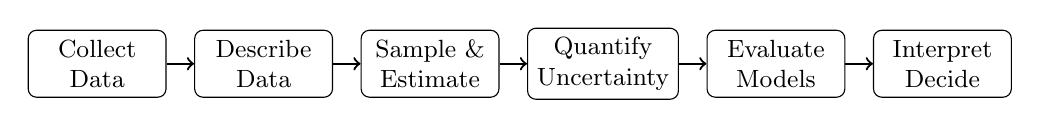
\begin{tikzpicture}[
    node distance=0.35cm,
    every node/.style={
        draw,
        rounded corners=3pt,
        align=center,
        minimum width=1.75cm,
        minimum height=0.85cm,
        font=\small
    },
    arrow/.style={->, thick}
]

\node (data) {Collect\\Data};

\node (describe) [right=of data]
    {Describe\\Data};

\node (estimate) [right=of describe]
    {Sample \&\\Estimate};

\node (uncertainty) [right=of estimate]
    {Quantify\\Uncertainty};

\node (model) [right=of uncertainty]
    {Evaluate\\Models};

\node (decision) [right=of model]
    {Interpret\\Decide};

\draw[arrow] (data) -- (describe);
\draw[arrow] (describe) -- (estimate);
\draw[arrow] (estimate) -- (uncertainty);
\draw[arrow] (uncertainty) -- (model);
\draw[arrow] (model) -- (decision);

\end{tikzpicture}

\end{center}

\vspace{0.35cm}

\begin{block}{Overall Idea}
\small
Descriptive statistics summarize observed data, while frequentist
methods use sampling and estimation to quantify uncertainty and
draw conclusions about population parameters.
\end{block}

\end{frame}
%-------------------------------------------------

\begin{frame}{Key Takeaways}

\begin{itemize}
    \item \textbf{Descriptive statistics} summarise the main features
          of observed data using numerical and graphical methods.

    \item \textbf{Histograms, moments and order statistics} help describe
          the distribution, centre and spread of data.

    \item \textbf{Covariance and covariance matrices} describe
          relationships and joint variability among variables.

    \item \textbf{Frequentist statistics} uses repeated sampling to
          estimate unknown population parameters.

    \item \textbf{MSE, bias, variance and consistency} are important
          properties for evaluating estimators.

    \item \textbf{Confidence intervals} quantify uncertainty in
          parameter estimates.

    \item \textbf{Parametric and non-parametric estimation} provide
          different approaches depending on distributional assumptions.

    \item These statistical concepts form an important foundation
          for \textbf{Data Science and AI}.
\end{itemize}

\end{frame}



\begin{frame}{References}

\begin{thebibliography}{9}

\bibitem{montgomery}
D. C. and G. C. Runger,
\textit{Applied Statistics and Probability for Engineers},
Wiley.

\bibitem{walpole}
R. E. et al.,
\textit{Probability and Statistics for Engineers and Scientists},
Pearson.

\bibitem{wasserman}
L. Wasserman,
\textit{All of Statistics: A Concise Course in Statistical Inference},
Springer.

\bibitem{james}
G. James et al.,
\textit{An Introduction to Statistical Learning},
Springer.

\bibitem{reference}
\textit{Descriptive and Frequentist Statistics},
Module 3 reference presentation.

\end{thebibliography}

\end{frame}


\end{document}